\documentclass[10pt,a4paper,onecolumn]{article}
\usepackage{marginnote}
\usepackage{graphicx}
\usepackage{xcolor}
\usepackage{authblk,etoolbox}
\usepackage{titlesec}
\usepackage{calc}
\usepackage{tikz}
\usepackage{hyperref}
\hypersetup{colorlinks,breaklinks,
            urlcolor=[rgb]{0.0, 0.5, 1.0},
            linkcolor=[rgb]{0.0, 0.5, 1.0}}
\usepackage{caption}
\usepackage{tcolorbox}
\usepackage{amssymb,amsmath}
\usepackage{ifxetex,ifluatex}
\usepackage{seqsplit}
\usepackage{fixltx2e} % provides \textsubscript
\usepackage[
  backend=biber,
%  style=alphabetic,
%  citestyle=numeric
]{biblatex}
\bibliography{paper.bib}


% --- Page layout -------------------------------------------------------------
\usepackage[top=3.5cm, bottom=3cm, right=1.5cm, left=1.0cm,
            headheight=2.2cm, reversemp, includemp, marginparwidth=4.5cm]{geometry}

% --- Default font ------------------------------------------------------------
% \renewcommand\familydefault{\sfdefault}

% --- Style -------------------------------------------------------------------
\renewcommand{\bibfont}{\small \sffamily}
\renewcommand{\captionfont}{\small\sffamily}
\renewcommand{\captionlabelfont}{\bfseries}

% --- Section/SubSection/SubSubSection ----------------------------------------
\titleformat{\section}
  {\normalfont\sffamily\Large\bfseries}
  {}{0pt}{}
\titleformat{\subsection}
  {\normalfont\sffamily\large\bfseries}
  {}{0pt}{}
\titleformat{\subsubsection}
  {\normalfont\sffamily\bfseries}
  {}{0pt}{}
\titleformat*{\paragraph}
  {\sffamily\normalsize}


% --- Header / Footer ---------------------------------------------------------
\usepackage{fancyhdr}
\pagestyle{fancy}
\fancyhf{}
%\renewcommand{\headrulewidth}{0.50pt}
\renewcommand{\headrulewidth}{0pt}
\fancyhead[L]{\hspace{-0.75cm}\includegraphics[width=5.5cm]{/Library/Frameworks/R.framework/Versions/4.1/Resources/library/rticles/rmarkdown/templates/joss/resources/JOSS-logo.png}}
\fancyhead[C]{}
\fancyhead[R]{}
\renewcommand{\footrulewidth}{0.25pt}

\fancyfoot[L]{\footnotesize{\sffamily , (2021). oce: an R package for
Oceanographic
Analysis. \textit{Journal of Open Source Software}, (), . \href{https://doi.org/}{https://doi.org/}}}


\fancyfoot[R]{\sffamily \thepage}
\makeatletter
\let\ps@plain\ps@fancy
\fancyheadoffset[L]{4.5cm}
\fancyfootoffset[L]{4.5cm}

% --- Macros ---------

\definecolor{linky}{rgb}{0.0, 0.5, 1.0}

\newtcolorbox{repobox}
   {colback=red, colframe=red!75!black,
     boxrule=0.5pt, arc=2pt, left=6pt, right=6pt, top=3pt, bottom=3pt}

\newcommand{\ExternalLink}{%
   \tikz[x=1.2ex, y=1.2ex, baseline=-0.05ex]{%
       \begin{scope}[x=1ex, y=1ex]
           \clip (-0.1,-0.1)
               --++ (-0, 1.2)
               --++ (0.6, 0)
               --++ (0, -0.6)
               --++ (0.6, 0)
               --++ (0, -1);
           \path[draw,
               line width = 0.5,
               rounded corners=0.5]
               (0,0) rectangle (1,1);
       \end{scope}
       \path[draw, line width = 0.5] (0.5, 0.5)
           -- (1, 1);
       \path[draw, line width = 0.5] (0.6, 1)
           -- (1, 1) -- (1, 0.6);
       }
   }

% --- Title / Authors ---------------------------------------------------------
% patch \maketitle so that it doesn't center
\patchcmd{\@maketitle}{center}{flushleft}{}{}
\patchcmd{\@maketitle}{center}{flushleft}{}{}
% patch \maketitle so that the font size for the title is normal
\patchcmd{\@maketitle}{\LARGE}{\LARGE\sffamily}{}{}
% patch the patch by authblk so that the author block is flush left
\def\maketitle{{%
  \renewenvironment{tabular}[2][]
    {\begin{flushleft}}
    {\end{flushleft}}
  \AB@maketitle}}
\makeatletter
\renewcommand\AB@affilsepx{ \protect\Affilfont}
%\renewcommand\AB@affilnote[1]{{\bfseries #1}\hspace{2pt}}
\renewcommand\AB@affilnote[1]{{\bfseries #1}\hspace{3pt}}
\makeatother
\renewcommand\Authfont{\sffamily\bfseries}
\renewcommand\Affilfont{\sffamily\small\mdseries}
\setlength{\affilsep}{1em}


\ifnum 0\ifxetex 1\fi\ifluatex 1\fi=0 % if pdftex
  \usepackage[T1]{fontenc}
  \usepackage[utf8]{inputenc}

\else % if luatex or xelatex
  \ifxetex
    \usepackage{mathspec}
  \else
    \usepackage{fontspec}
  \fi
  \defaultfontfeatures{Ligatures=TeX,Scale=MatchLowercase}

\fi
% use upquote if available, for straight quotes in verbatim environments
\IfFileExists{upquote.sty}{\usepackage{upquote}}{}
% use microtype if available
\IfFileExists{microtype.sty}{%
\usepackage{microtype}
\UseMicrotypeSet[protrusion]{basicmath} % disable protrusion for tt fonts
}{}

\usepackage{hyperref}
\hypersetup{unicode=true,
            pdftitle={oce: an R package for Oceanographic Analysis},
            pdfborder={0 0 0},
            breaklinks=true}
\urlstyle{same}  % don't use monospace font for urls
\usepackage{color}
\usepackage{fancyvrb}
\newcommand{\VerbBar}{|}
\newcommand{\VERB}{\Verb[commandchars=\\\{\}]}
\DefineVerbatimEnvironment{Highlighting}{Verbatim}{commandchars=\\\{\}}
% Add ',fontsize=\small' for more characters per line
\usepackage{framed}
\definecolor{shadecolor}{RGB}{248,248,248}
\newenvironment{Shaded}{\begin{snugshade}}{\end{snugshade}}
\newcommand{\AlertTok}[1]{\textcolor[rgb]{0.94,0.16,0.16}{#1}}
\newcommand{\AnnotationTok}[1]{\textcolor[rgb]{0.56,0.35,0.01}{\textbf{\textit{#1}}}}
\newcommand{\AttributeTok}[1]{\textcolor[rgb]{0.77,0.63,0.00}{#1}}
\newcommand{\BaseNTok}[1]{\textcolor[rgb]{0.00,0.00,0.81}{#1}}
\newcommand{\BuiltInTok}[1]{#1}
\newcommand{\CharTok}[1]{\textcolor[rgb]{0.31,0.60,0.02}{#1}}
\newcommand{\CommentTok}[1]{\textcolor[rgb]{0.56,0.35,0.01}{\textit{#1}}}
\newcommand{\CommentVarTok}[1]{\textcolor[rgb]{0.56,0.35,0.01}{\textbf{\textit{#1}}}}
\newcommand{\ConstantTok}[1]{\textcolor[rgb]{0.00,0.00,0.00}{#1}}
\newcommand{\ControlFlowTok}[1]{\textcolor[rgb]{0.13,0.29,0.53}{\textbf{#1}}}
\newcommand{\DataTypeTok}[1]{\textcolor[rgb]{0.13,0.29,0.53}{#1}}
\newcommand{\DecValTok}[1]{\textcolor[rgb]{0.00,0.00,0.81}{#1}}
\newcommand{\DocumentationTok}[1]{\textcolor[rgb]{0.56,0.35,0.01}{\textbf{\textit{#1}}}}
\newcommand{\ErrorTok}[1]{\textcolor[rgb]{0.64,0.00,0.00}{\textbf{#1}}}
\newcommand{\ExtensionTok}[1]{#1}
\newcommand{\FloatTok}[1]{\textcolor[rgb]{0.00,0.00,0.81}{#1}}
\newcommand{\FunctionTok}[1]{\textcolor[rgb]{0.00,0.00,0.00}{#1}}
\newcommand{\ImportTok}[1]{#1}
\newcommand{\InformationTok}[1]{\textcolor[rgb]{0.56,0.35,0.01}{\textbf{\textit{#1}}}}
\newcommand{\KeywordTok}[1]{\textcolor[rgb]{0.13,0.29,0.53}{\textbf{#1}}}
\newcommand{\NormalTok}[1]{#1}
\newcommand{\OperatorTok}[1]{\textcolor[rgb]{0.81,0.36,0.00}{\textbf{#1}}}
\newcommand{\OtherTok}[1]{\textcolor[rgb]{0.56,0.35,0.01}{#1}}
\newcommand{\PreprocessorTok}[1]{\textcolor[rgb]{0.56,0.35,0.01}{\textit{#1}}}
\newcommand{\RegionMarkerTok}[1]{#1}
\newcommand{\SpecialCharTok}[1]{\textcolor[rgb]{0.00,0.00,0.00}{#1}}
\newcommand{\SpecialStringTok}[1]{\textcolor[rgb]{0.31,0.60,0.02}{#1}}
\newcommand{\StringTok}[1]{\textcolor[rgb]{0.31,0.60,0.02}{#1}}
\newcommand{\VariableTok}[1]{\textcolor[rgb]{0.00,0.00,0.00}{#1}}
\newcommand{\VerbatimStringTok}[1]{\textcolor[rgb]{0.31,0.60,0.02}{#1}}
\newcommand{\WarningTok}[1]{\textcolor[rgb]{0.56,0.35,0.01}{\textbf{\textit{#1}}}}
\usepackage{graphicx,grffile}
\makeatletter
\def\maxwidth{\ifdim\Gin@nat@width>\linewidth\linewidth\else\Gin@nat@width\fi}
\def\maxheight{\ifdim\Gin@nat@height>\textheight\textheight\else\Gin@nat@height\fi}
\makeatother
% Scale images if necessary, so that they will not overflow the page
% margins by default, and it is still possible to overwrite the defaults
% using explicit options in \includegraphics[width, height, ...]{}
\setkeys{Gin}{width=\maxwidth,height=\maxheight,keepaspectratio}
\IfFileExists{parskip.sty}{%
\usepackage{parskip}
}{% else
\setlength{\parindent}{0pt}
\setlength{\parskip}{6pt plus 2pt minus 1pt}
}
\setlength{\emergencystretch}{3em}  % prevent overfull lines
\providecommand{\tightlist}{%
  \setlength{\itemsep}{0pt}\setlength{\parskip}{0pt}}
\setcounter{secnumdepth}{0}
% Redefines (sub)paragraphs to behave more like sections
\ifx\paragraph\undefined\else
\let\oldparagraph\paragraph
\renewcommand{\paragraph}[1]{\oldparagraph{#1}\mbox{}}
\fi
\ifx\subparagraph\undefined\else
\let\oldsubparagraph\subparagraph
\renewcommand{\subparagraph}[1]{\oldsubparagraph{#1}\mbox{}}
\fi

% Pandoc citation processing
\newlength{\csllabelwidth}
\setlength{\csllabelwidth}{3em}
\newlength{\cslhangindent}
\setlength{\cslhangindent}{1.5em}
% for Pandoc 2.8 to 2.10.1
\newenvironment{cslreferences}%
  {}%
  {\par}
% For Pandoc 2.11+
\newenvironment{CSLReferences}[3] % #1 hanging-ident, #2 entry spacing
 {% don't indent paragraphs
  \setlength{\parindent}{0pt}
  % turn on hanging indent if param 1 is 1
  \ifodd #1 \everypar{\setlength{\hangindent}{\cslhangindent}}\ignorespaces\fi
  % set entry spacing
  \ifnum #2 > 0
  \setlength{\parskip}{#2\baselineskip}
  \fi
 }%
 {}
\usepackage{calc} % for calculating minipage widths
\newcommand{\CSLBlock}[1]{#1\hfill\break}
\newcommand{\CSLLeftMargin}[1]{\parbox[t]{\csllabelwidth}{#1}}
\newcommand{\CSLRightInline}[1]{\parbox[t]{\linewidth - \csllabelwidth}{#1}}
\newcommand{\CSLIndent}[1]{\hspace{\cslhangindent}#1}


\title{oce: an R package for Oceanographic Analysis}

        \author[1]{Dan E. Kelley\footnote{Corresponding author.}}
          \author[2]{Clark Richards}
          \author[3]{Chantelle Layton}
    
      \affil[1]{Dan E. Kelley, Professor, Dalhousie University}
      \affil[2]{Clark Richards, Research Scientist, Bedford Institute of
Oceanography, Department of Fisheries and Oceans, Canada; also Adjunct
Professor, Dalhousie University}
      \affil[3]{Chantelle Layton, Physical Scientist, Bedford Institute
of Oceanography, Department of Fisheries and Oceans, Canada}
  \date{\vspace{-5ex}}

\begin{document}
\maketitle

\marginpar{
  %\hrule
  \sffamily\small

  {\bfseries DOI:} \href{https://doi.org/}{\color{linky}{}}

  \vspace{2mm}

  {\bfseries Software}
  \begin{itemize}
    \setlength\itemsep{0em}
    \item \href{}{\color{linky}{Review}} \ExternalLink
    \item \href{}{\color{linky}{Repository}} \ExternalLink
    \item \href{}{\color{linky}{Archive}} \ExternalLink
  \end{itemize}

  \vspace{2mm}

  {\bfseries Submitted:} \\
  {\bfseries Published:} 

  \vspace{2mm}
  {\bfseries License}\\
  Authors of papers retain copyright and release the work under a Creative Commons Attribution 4.0 International License (\href{http://creativecommons.org/licenses/by/4.0/}{\color{linky}{CC-BY}}).
}

\hypertarget{statement-of-need}{%
\section{Statement of Need}\label{statement-of-need}}

Oceanographic field experiments often employ a wide variety of
instrument types, each of which reports data in an individual format.
Many of these formats are quite complex, and decoding them can be a
challenge, partly owing to weaknesses in the documentation provided by
manufacturers. Although manufacturers tend to provide software for
viewing data from their instruments, it is usually proprietary and
closed-source, which does not help researchers who need to investigate
the data in new ways, and to combine data from multiple instruments. The
\texttt{oce} package (Kelley, Richards, \& Layton, 2021) was developed
to simplify data input, and to do so in an integrated way that
facilitates open-ended analysis that employs multiple data types. It
also provides tools for undertaking specialized oceanographic
calculations (e.g., relating to seawater properties) and providing
graphical displays that follow oceanographic conventions. This is all
done in the R language (Ihaka \& Gentleman, 1996; R Core Team, 2021),
which provides wide-ranging data analysis tools that are needed for
oceanographic research (Kelley, 2018).

\hypertarget{overview}{%
\section{Overview}\label{overview}}

The \texttt{oce} package has been hosted on CRAN ({``The {Comprehensive}
{R} {Archive} {Network},''} 2021) since the year 2009. The CRAN version,
which is updated once or twice a year, may be installed by typing
\texttt{install.packages("oce")} in an R console. Users who need newer
features may use
\texttt{remotes::install\_github("dankelley/oce",ref="develop")} to
download and build the development branch. Those wishing to investigate
or participate in the development process are welcome to do so, at
\url{https://github.com/dankelley/oce}.

The package has functions for decoding a long list of
instrument-specific data formats. The return values of those functions
are expressed in the S4 object-orientation scheme, with slots for (a)
the actual data, (b) related metadata, and (c) a log of the \texttt{oce}
function calls used in creating the object. This is illustrated by the
results of executing the following in an R session, for the case of an
object of the \texttt{"ctd"} subclass, which holds data acquired from a
CTD (Conductivity-Depth-Pressure) instrument, a workhorse of
oceanographic sampling.

\begin{Shaded}
\begin{Highlighting}[]
\FunctionTok{library}\NormalTok{(oce)                           }\CommentTok{\# load library}
\FunctionTok{data}\NormalTok{(ctd)                              }\CommentTok{\# load a built{-}in sample file}
\FunctionTok{slotNames}\NormalTok{(ctd)                         }\CommentTok{\# see \textquotesingle{}slot\textquotesingle{} names}
\end{Highlighting}
\end{Shaded}

The last function call shown above is provided to explain the structure,
but it is seldom used in practice. Rather, the next step after loading
an object, or reading it from a data file, is often to view textual and
graphical summaries of the data, with

\begin{Shaded}
\begin{Highlighting}[]
\FunctionTok{summary}\NormalTok{(ctd)                           }\CommentTok{\# results not shown here}
\FunctionTok{plot}\NormalTok{(ctd)                              }\CommentTok{\# results in Figure 1}
\end{Highlighting}
\end{Shaded}

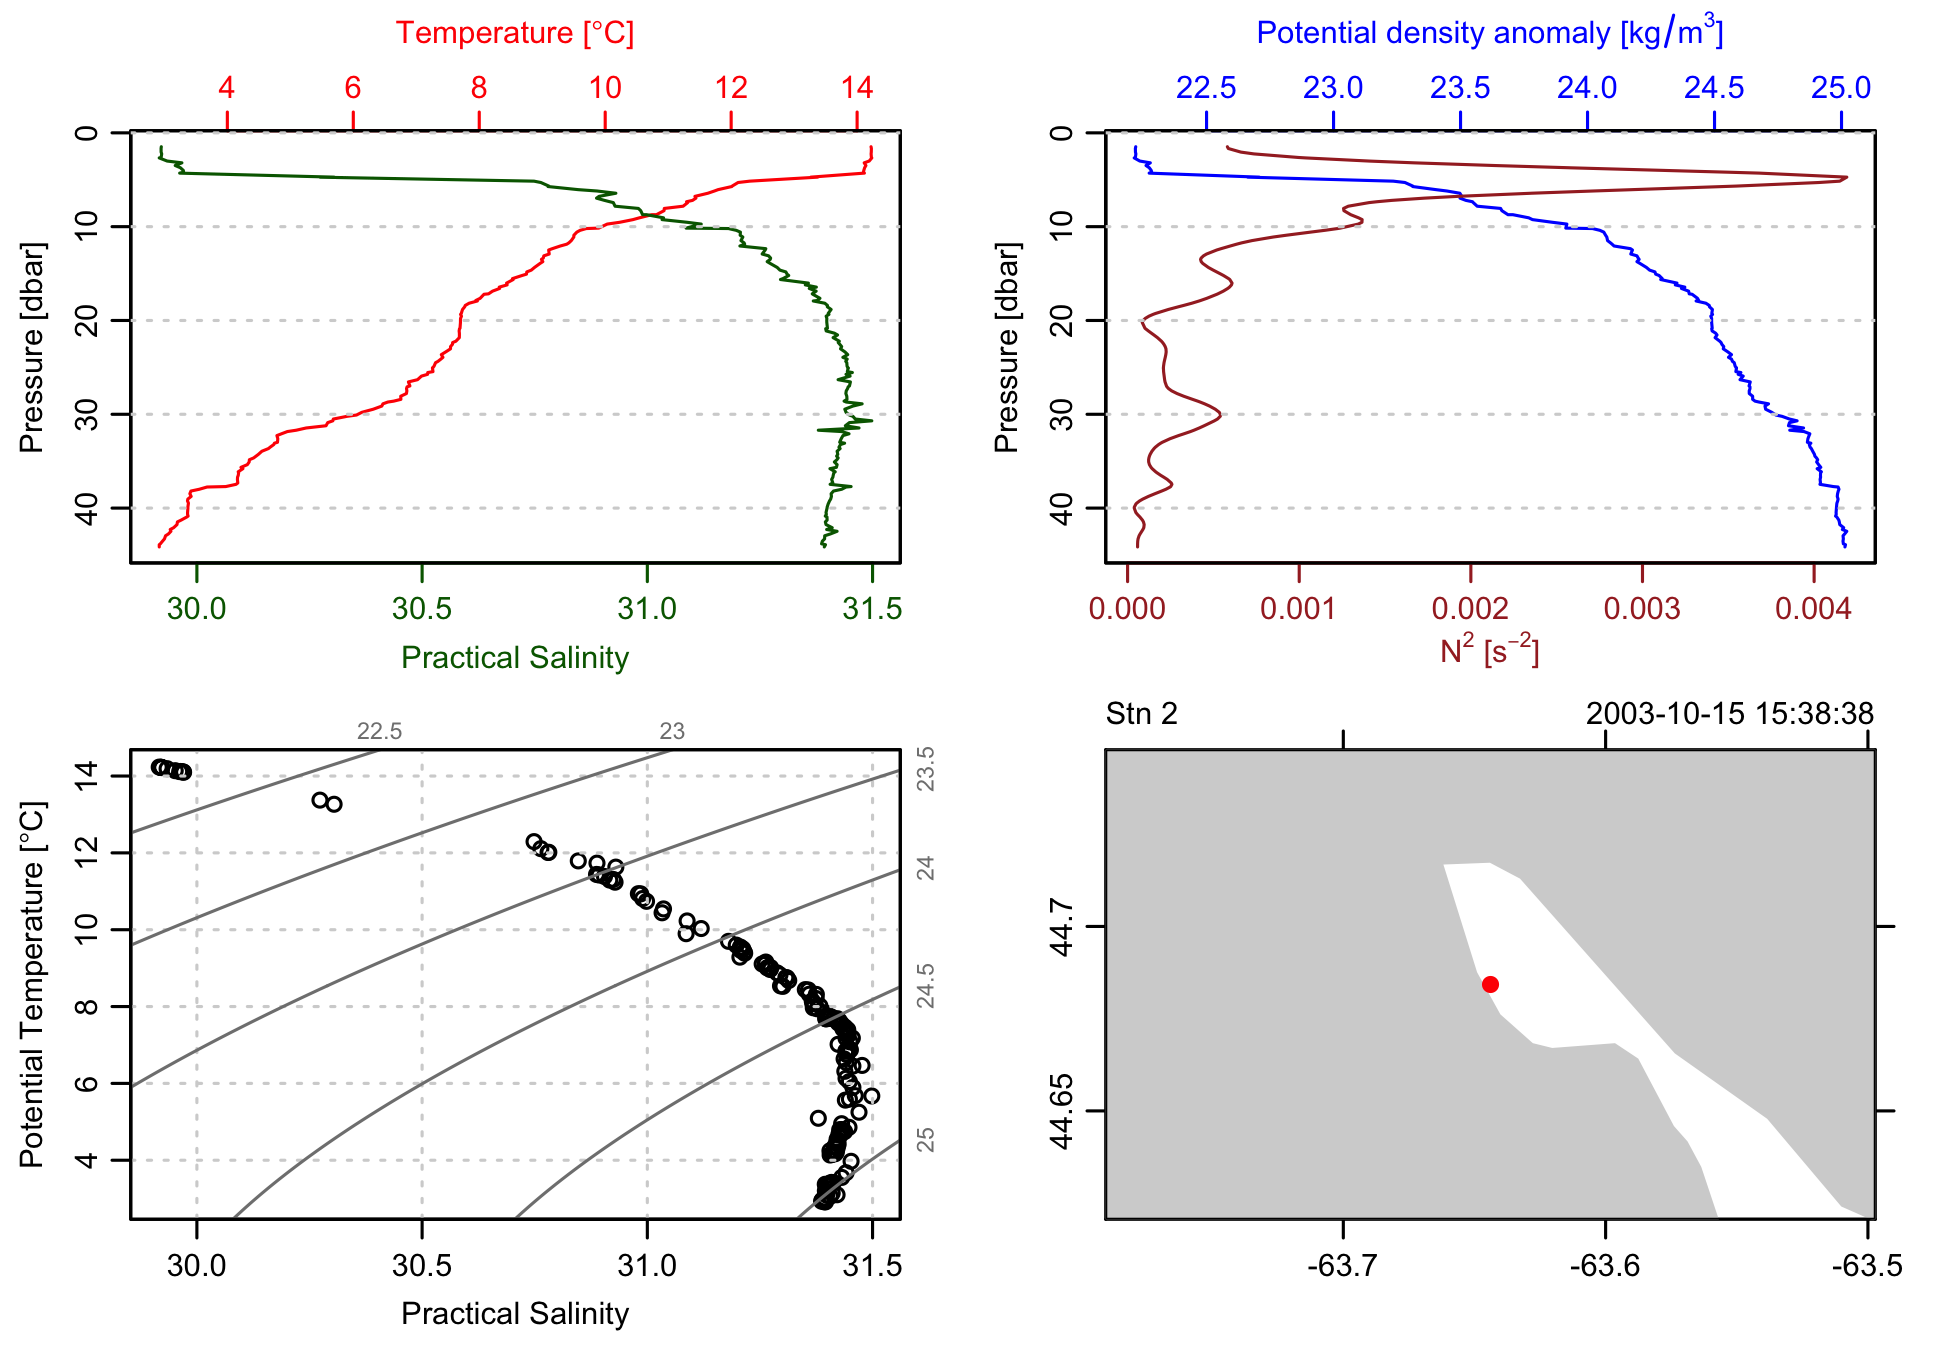
\includegraphics{unnamed-chunk-2-1.png} the latter of which produces
Figure 1. This diagram is good for an overview, but \texttt{oce} also
provides more fine-grained control of graphical representations, with
e.g.

\begin{Shaded}
\begin{Highlighting}[]
\FunctionTok{plot}\NormalTok{(ctd, }\AttributeTok{which=}\StringTok{"temperature"}\NormalTok{)}
\end{Highlighting}
\end{Shaded}

plotting just temperature variation with depth (results not shown here).
The variations of other properties may be shown by setting
\texttt{which} appropriately, and this argument can also be used to
specify other types of plots, in addition to the depth-variation form.

Besides this \texttt{"ctd"} subclass, \texttt{oce} supports over two
dozen other subclasses that cover a wide range of oceanographic
instrumentation. In every case, the same \texttt{"summary()"} and
\texttt{"plot()"} function calls provide textual and graphical
representations of the contents of the object. This specialization of
these two generic functions simplifies analysis considerably. For
example, if \texttt{PATTERN} is a regular expression that specifies a
set of data files, whether of a single instrument type or multiple
instrument types, then

\begin{Shaded}
\begin{Highlighting}[]
\ControlFlowTok{for}\NormalTok{ (file }\ControlFlowTok{in} \FunctionTok{list.files}\NormalTok{(PATTERN)) \{}
\NormalTok{    d }\OtherTok{\textless{}{-}} \FunctionTok{read.oce}\NormalTok{(file)}
    \FunctionTok{summary}\NormalTok{(d)}
    \FunctionTok{plot}\NormalTok{(d)}
\NormalTok{\}}
\end{Highlighting}
\end{Shaded}

will provide information about each data file of interest, forming a
good first stage of analysis. More detailed plot calls are usually
required for the second stage of analysis, but a feature of \texttt{oce}
(and R) is that it is often quite easy to undertake such analyses.

Oce provides other generic functions, such as \texttt{subset()} for
focusing on subsets of data, \texttt{handleFlags()} for processing
data-quality flags, and \texttt{{[}{[}} for accessing data. This
accessor operation is particularly worthy of note, for several reasons,
of which two stand out.

\begin{enumerate}
\def\labelenumi{\arabic{enumi}.}
\item
  \texttt{{[}{[}} lets users access information regardless of where it
  occurs in the object. For example, a CTD does not measure longitude
  and latitude, but these things are often streamed into data files
  separately, so they are stored in the object's \texttt{metadata} slot,
  not the \texttt{data} slot. Users do not need to know this detail,
  though, because e.g.~\texttt{ctd{[}{[}"longitude"{]}{]}} will extract
  longitude from whichever slot holds it. For other data types,
  e.g.~from a GPS instrument, the \texttt{{[}{[}} operation would get it
  from the \texttt{data} slot. Importantly, a single line of code would
  work for both types of data, so, again, code written for one object
  type will work for another.
\item
  \texttt{{[}{[}} can access not just information stored within the
  object, but also things that can be calculated from that information.
  For example, CTD files typically hold temperature along with other
  properties from which seawater density may be computed (McDougall \&
  Barker, 2011; Millero, 2010). Density is an important dynamical
  factor, and so \texttt{oce} is set up so that e.g.
  \texttt{ctd{[}{[}"density"{]}{]}} will compute it, if the object named
  \texttt{ctd} contains the required elements. This also applies for
  other elements that are commonly needed for oceanographic analysis,
  but not measured directly.
\end{enumerate}

The significance of \texttt{{[}{[}} is that it forms a bridge from the
oceanographic realm to the general R realm, letting users extract the
data into whatever form will facilitate further analysis. With tens of
thousands of well-vetted R packages covering a wide array of statistical
and other methods, this lets oceanographers focus on their work, not on
tool generation.

\hypertarget{example-tidal-analysis}{%
\section{Example: Tidal Analysis}\label{example-tidal-analysis}}

A more detailed example may help to solidify some of the key aspects of
\texttt{oce}. Many readers will have an interest in tides, so we will
work with a year-long record of sea level, \(\eta=\eta(t)\) in Halifax
Harbour, in the year 2003, during which the city was struck by Hurricane
Juan.

Consider the code given below, which produces Figure 2. Comments made
within the code ought to be reasonably self-explanatory. A built-in
sealevel file is used, to make a reproducible example, but replacing the
\texttt{data()} call with a \texttt{read.sealevel()} call will handle
data files in standard formats. Note that the \texttt{tidem()} function
is quite sophisticated, covering over 500 lines of R code in order to
apply specialized procedures developed in the tidal-research community
(Foreman, Cherniawsky, \& Ballantyne, 2009; Godin, 1972; Pawlowicz,
Beardsley, \& Lentz, 2002). Readers with R experience may notice that
the function name evoke the \texttt{lm()} function for linear models,
and they may not be surprised that \texttt{oce} provides a function
named \texttt{predict()}, for generating tidal predictions from tidal
models.

\begin{Shaded}
\begin{Highlighting}[]
\FunctionTok{library}\NormalTok{(oce)                           }\CommentTok{\# load library}
\FunctionTok{data}\NormalTok{(sealevel)                         }\CommentTok{\# use built{-}in example dataset}
\NormalTok{t }\OtherTok{\textless{}{-}}\NormalTok{ sealevel[[}\StringTok{"time"}\NormalTok{]]                }\CommentTok{\# extract time}
\NormalTok{eta }\OtherTok{\textless{}{-}}\NormalTok{ sealevel[[}\StringTok{"elevation"}\NormalTok{]]         }\CommentTok{\# extract sea level}
\NormalTok{m }\OtherTok{\textless{}{-}} \FunctionTok{tidem}\NormalTok{(sealevel)                   }\CommentTok{\# fit tidal model}
\NormalTok{etaDetided }\OtherTok{\textless{}{-}}\NormalTok{ eta }\SpecialCharTok{{-}} \FunctionTok{predict}\NormalTok{(m)         }\CommentTok{\# de{-}tide observations}
\FunctionTok{par}\NormalTok{(}\AttributeTok{mfrow=}\FunctionTok{c}\NormalTok{(}\DecValTok{2}\NormalTok{, }\DecValTok{1}\NormalTok{))                     }\CommentTok{\# set up a two{-}panel plot}
\FunctionTok{oce.plot.ts}\NormalTok{(t, eta, }\AttributeTok{xaxs=}\StringTok{"i"}\NormalTok{,          }\CommentTok{\# top: observed sea level}
    \AttributeTok{grid=}\ConstantTok{TRUE}\NormalTok{, }\AttributeTok{ylab=}\StringTok{"Sea level [m]"}\NormalTok{)}
\FunctionTok{oce.plot.ts}\NormalTok{(t, etaDetided, }\AttributeTok{xaxs=}\StringTok{"i"}\NormalTok{,   }\CommentTok{\# bottom: de{-}tided sea level}
    \AttributeTok{grid=}\ConstantTok{TRUE}\NormalTok{, }\AttributeTok{ylab=}\StringTok{"De{-}tided sea level [m]"}\NormalTok{)}
\end{Highlighting}
\end{Shaded}

\begin{figure}
\centering
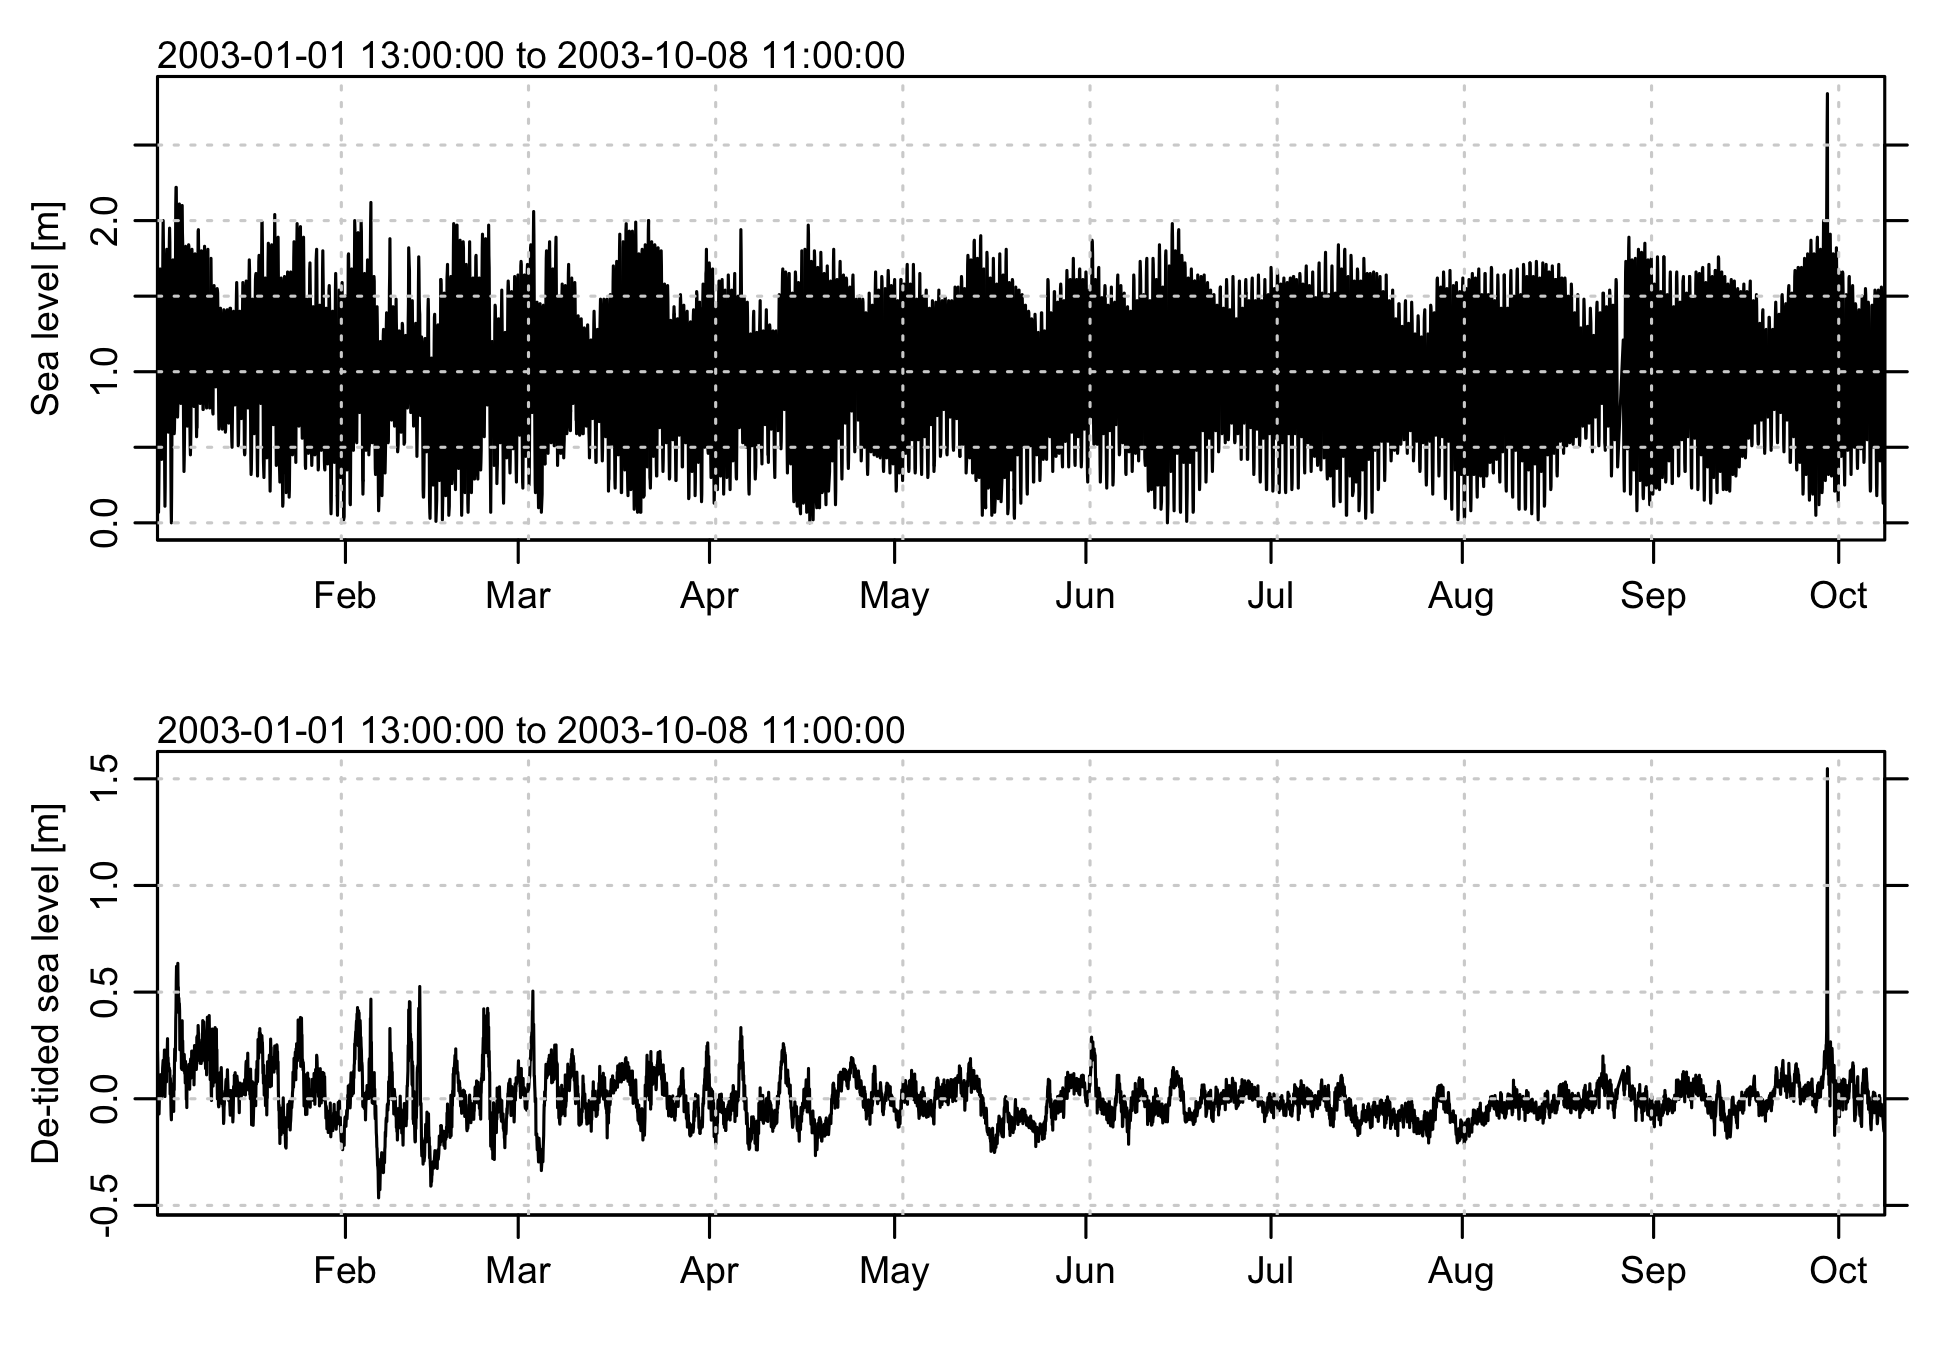
\includegraphics{unnamed-chunk-5-1.png}
\caption{Tidal analysis example. Top: a year of sea level variation in
Halifax Harbour. Bottom: sea level after removing a fit to the tides.}
\end{figure}

A comparison of the panels of Figure 2 reveals that tides explain much
of the sea level variation in Halifax Harbour. The lower panel
illustrates an increase of detided variance during the winter months, as
is expected for a site at a northern mid-latitude. More surprising is
the large spike towards the end of September. This is a result of
Hurricane Juan, which swept over Halifax at that time, causing a storm
surge of in sea level amounting to approximately 1.5m that, along with
high waves, caused major damage in the harbour (Xu \& Perrie, 2012).
(Readers with an interest might find it informative to supply an
\texttt{xlim} argument to the plot calls, to narrow in on the event.)

\hypertarget{conclusions}{%
\section{Conclusions}\label{conclusions}}

The \texttt{oce} package provides for many aspects of oceanographic
analysis, having evolved in an open-source environment for more than a
decade. The developers have benefited from a supportive user community,
members of which have contributed insightful bug reports and suggestions
for improvements. New features are added continually, to handle new
instrument types, new data repositories, and new methods. Physical
oceanography is a major focus of the package, but our goal in writing
this paper is to develop interest from other communities, ranging from
climatologists to those in marine disciplines such as chemistry and
biology. We also hope to encourage and facilitate new R packages, such
as \texttt{argoFloats} (Kelley, Harbin, \& Richards, 2021), that build
upon \texttt{oce}.

\hypertarget{references}{%
\section*{References}\label{references}}
\addcontentsline{toc}{section}{References}

\hypertarget{refs}{}
\begin{CSLReferences}{1}{0}
\leavevmode\vadjust pre{\hypertarget{ref-foreman_versatile_2009}{}}%
Foreman, M. G. G., Cherniawsky, J. Y., \& Ballantyne, V. A. (2009).
Versatile harmonic tidal analysis: {Improvements} and applications.
\emph{Journal of Atmospheric and Oceanic Technology}, \emph{26}(4),
806--817.
doi:\href{https://doi.org/10.1175/2008JTECHO615.1}{10.1175/2008JTECHO615.1}

\leavevmode\vadjust pre{\hypertarget{ref-godin_analysis_1972}{}}%
Godin, G. (1972). \emph{The {Analysis} of {Tides}}. Toronto: University
of Toronto Press.

\leavevmode\vadjust pre{\hypertarget{ref-ihaka_r_1996}{}}%
Ihaka, R., \& Gentleman, R. (1996). R: {A} {Language} for {Data}
{Analysis} and {Graphics}. \emph{Journal of Computational \& Graphical
Statistics}, \emph{5}(3), pp. 299--314. Retrieved from
\url{http://www.jstor.org/stable/1390807}

\leavevmode\vadjust pre{\hypertarget{ref-kelley_oceanographic_2018}{}}%
Kelley, D. E. (2018). \emph{Oceanographic {Analysis} with {R}}. New
York: Springer-Verlag.

\leavevmode\vadjust pre{\hypertarget{ref-kelley_argofloats_2021}{}}%
Kelley, D. E., Harbin, J., \& Richards, C. (2021). {argoFloats}: {An}
{R} {Package} for {Analyzing} {Argo} {Data}. \emph{Frontiers in Marine
Science}, \emph{8}, 409.
doi:\href{https://doi.org/10.3389/fmars.2021.635922}{10.3389/fmars.2021.635922}

\leavevmode\vadjust pre{\hypertarget{ref-kelley__aut_oce_2021}{}}%
Kelley, D. E., Richards, C., \& Layton, C. (2021, March). Oce:
{Analysis} of {Oceanographic} {Data}. Retrieved from
\url{https://CRAN.R-project.org/package=oce}

\leavevmode\vadjust pre{\hypertarget{ref-mcdougall_getting_2011}{}}%
McDougall, T. J., \& Barker, P. M. (2011). \emph{Getting started with
{TEOS}-10 and the {Gibbs} {Seawater} ({GSW}) {Oceanographic} {Toolbox}}.
SCOR/IAPSO WG127.

\leavevmode\vadjust pre{\hypertarget{ref-millero_history_2010}{}}%
Millero, F. (2010). History of the {Equation} of {State} of {Seawater}.
\emph{Oceanography}, \emph{23}(3), 18--33.
doi:\href{https://doi.org/10.5670/oceanog.2010.21}{10.5670/oceanog.2010.21}

\leavevmode\vadjust pre{\hypertarget{ref-pawlowicz_classical_2002}{}}%
Pawlowicz, R., Beardsley, B., \& Lentz, S. (2002). Classical tidal
harmonic analysis including error estimates in {MATLAB} using {T}\_TIDE.
\emph{Computers \& Geosciences}, \emph{28}(8), 929--937.
doi:\href{https://doi.org/10.1016/S0098-3004(02)00013-4}{10.1016/S0098-3004(02)00013-4}

\leavevmode\vadjust pre{\hypertarget{ref-r_core_team_introduction_2021}{}}%
R Core Team. (2021). An {Introduction} to {R}. Retrieved from
\url{https://cran.r-project.org/doc/manuals/r-release/R-intro.html}

\leavevmode\vadjust pre{\hypertarget{ref-noauthor_comprehensive_2021}{}}%
The {Comprehensive} {R} {Archive} {Network}. (2021, January). Retrieved
from \url{https://cran.r-project.org/}

\leavevmode\vadjust pre{\hypertarget{ref-xu_extreme_2012}{}}%
Xu, F., \& Perrie, W. (2012). Extreme {Waves} and {Wave} {Run}-up in
{Halifax} {Harbour} under {Climate} {Change} {Scenarios}.
\emph{Atmosphere-Ocean}, \emph{50}(4), 407--420.
doi:\href{https://doi.org/10.1080/07055900.2012.707610}{10.1080/07055900.2012.707610}

\end{CSLReferences}

\end{document}
